%----------------------------------------------------------------------------------------
%	CHAPTER - DEVELOPMENT
%----------------------------------------------------------------------------------------

\chapter{Development}

\label{ChapterDevelopment}

% ################################################################
\definecolor{bluekeywords}{rgb}{0,0,1}
\definecolor{greencomments}{rgb}{0,0.5,0}
\definecolor{redstrings}{rgb}{0.64,0.08,0.08}
\definecolor{xmlcomments}{rgb}{0.5,0.5,0.5}
\definecolor{types}{rgb}{0.17,0.57,0.68}

\lstset{language=[Sharp]C,
	captionpos=b,
	%numbers=left, %Nummerierung
	%numberstyle=\tiny, % kleine Zeilennummern
	frame=lines, % Oberhalb und unterhalb des Listings ist eine Linie
	showspaces=false,
	showtabs=false,
	breaklines=true,
	showstringspaces=false,
	breakatwhitespace=true,
	escapeinside={(*@}{@*)},
	commentstyle=\color{greencomments},
	morekeywords={partial, var, value, get, set},
	keywordstyle=\color{bluekeywords},
	stringstyle=\color{redstrings},
	basicstyle=\ttfamily\small,
}
% ################################################################

%----------------------------------------------------------------------------------------
%	SECTION 1
%----------------------------------------------------------------------------------------

\section{Introduction}

The \textit{Development} phase, as defined by \cite{Vaishnavi2008} and \cite{Hevner2010}, comes after the \textit{Suggestion} of a design and focuses on the further development and implementation of the design. The outcome of this chapter is the requirement for the subsequent \textit{Evaluation} chapter. This is a crucial step in answering \gls{srq} 4 since the to be achieved benefits over the traditional approaches have only been of theoretical nature so far, but are not tested for their feasibility yet. \cite{Vaishnavi2008} see different techniques on how the implementation can look like, depending on the to be constructed artifact. For this thesis, the development of a prototype application in \gls{vr} has been chosen. In a first step, the technical setup is defined, before the architecture and data model for the prototype are discussed. Following that, the actual implementation of the different views and navigations are covered with a conclusion at the end. \newline
Building up on this, the \textit{Evaluation} phase will then be discussed in chapter \ref{ChapterEvaluation}.


%----------------------------------------------------------------------------------------
%	SECTION 2
%----------------------------------------------------------------------------------------

\section{Technical Setup}

The technical setup chapter gives a description and explanation for the selection of the individual components that are used for the development of the prototype application. It can be distinguished between Hardware and Software components that are discussed in their respective sub-chapters.


%-----------------------------------
%	SUBSECTION 1
%-----------------------------------
\subsection{Hardware}

The in the literature review discussed different methods for user input as part of \gls{srq} 2 have been summarized in table \ref{tbl:methodscomparison}. For the selection of the right \gls{vr} device, this conclusion was considered for the evaluation. While for the \textit{Travel} aspect only three methods (including the option for no travel at all) have been discussed:

\textbf{No travelling option:}
By looking at \gls{mdg} 2 that defines the user to be part of the \gls{ve} and thus is able to 'travel' around the visualisations, the third option would violate this design goal and thus is no viable option.

\textbf{Full Body Tracking:}
While it allows for free movement within \gls{ve}, it is lacking accuracy and only works from one angle. This can be effectively used if a static display in one direction is used which updates the data that it displays. With an implementation of the 'multiples linked views' concept however, one angle will not be enough anymore.

\textbf{360° Motion Tracking:}
Compared to 'Full Body Tracking', the '360° Motion Tracking' provides much better accuracy and allows for spatial positioning in all three axis, which strongly supports \gls{mdg} 2.


This leads to a first conclusion for '360° Motion Tracking' which is the only methods for \textit{Travel} that fulfils all requirements of the design goals. For \textit{Selection} (and \textit{Manipulation}), some more methods had been discussed:

\textbf{No selection/manipulation option:}
The option for no input method cannot be considered as the application would then provide no interaction at all and thus violate \gls{mdg} 1 that requires a high interactivity with tightly coupled actions/reactions.

\textbf{Hand Gestures:}
While 'Hand Gestures' offer a very high familiarity, they have a limited tracking area and become less accurate with faster movements. Although the latter is not of that importance, the limited tracking area can become problematic with the different views, especially since the supporting views are placed in the centre of where the user is looking at.

\textbf{Gesture Controllers:}
TODO: tbd

\textbf{Speech Recognition:}
This methods requires a silent area and good pronunciation of one of the supported official languages, as dialects can be quite problematic. While it allows for some very interesting, more complex queries such as "Show me all transactions in the last seven days over CHF 100.", it rather can be seen as a supportive input method, but not as the main input method.

\textbf{Physical Placement of Objects:}
While the 'Physical Placement of Objects' would be the most realistic and immersive option, it can be considered as to expensive and also too difficult to build as for this design goal not only some buttons and knobs would need to be built, but also fully dynamic charts and tables.


It can be concluded, that the 'Gesture Controllers' have the highest fit, and also work very well together with the '360° Motion Tracking'. Speech Recognition can provide some interesting support-functionalities that should be looked at in future research. \newline
This combination of input methods are best met with the HTC Vive (\url{https://www.vive.com/}) that was unveiled by HTC in early 2016. The bundle consists of a \gls{hmd}, two gesture controllers (as explained in Chapter \ref{SubSubSectionGestureControllers}) and two so called 'Lighthouses' (as explained in Chapter \ref{360MotionTracking}) that when set up in opposite corner allow for a full motion tracking.


%-----------------------------------
%	SUBSECTION 2
%-----------------------------------

\subsection{Software}

All used software for the development of the \gls{vr} prototype is summarised and described in the following sub-chapters.


\subsubsection{Game Engine}
At the foundation, the multi-platform game engine and development toolkit 'Unity 3D' is used. It offers the option to not only develop 2D, but also 3D applications that can be run in \gls{vr}. It is used for the actual design of the \gls{ve}, and the placement and configuration of 3D objects.

\textbf{Software:} Unity 3D \newline
\textbf{Version:} 5.5.0f3 \newline
\textbf{Publisher:} \cite{Unity2016} \newline
\textbf{Link:} \url{http://unity3d.com/}


\subsubsection{Game Engine Plugins}
For the integration of the \gls{sdk} to access the specific methods and functions of the HTC Vive, the SteamVR plugin for Unity is used. In addition to this, \gls{vrtk} will be used as a toolkit to rely on 'semi-standardised' ways for certain \gls{vr}-specific interactions and functions in Unity 3D. Even though the HTC Vive has been chosen for the hardware part, due to the usage of the SteamVR plugin and the \gls{vrtk}, only little to none changes should be required in order to have the prototype application also run other supported hardware such as the Oculus Rift, since both of them support multiple \glspl{hmd}.

\textbf{Software:} SteamVR Plugin \newline
\textbf{Version:} 1.1.1 \newline
\textbf{Publisher:} \cite{Valve2016a} \newline
\textbf{Link:} \url{https://www.assetstore.unity3d.com/en/#!/content/32647}

\textbf{Software:} \gls{vrtk} - Virtual Reality Toolkit \newline
\textbf{Version:} 3.0.0 \newline
\textbf{Publisher:} \cite{Sysdia2017} \newline
\textbf{Link:} \url{https://www.assetstore.unity3d.com/en/#!/content/64131} \newline
\textbf{Link:} \url{https://vrtoolkit.readme.io/}


\subsubsection{\gls{ide}}
Microsoft Visual Studio Community 2015 from  is used for the development of the Unity Scripts in the programming language C\#. These scripts handle and manage the whole \gls{ve} by triggering interactions of the 3D objects defined and placed in Unity 3D.

\textbf{Software:} Microsoft Visual Studio Community \newline
\textbf{Version:} 2015 \newline
\textbf{Publisher:} \cite{Microsoft2015} \newline
\textbf{Link:} \url{https://www.microsoft.com/en-us/download/details.aspx?id=48146}
 

\subsubsection{3D Graphics}

Finally, for the design of custom 3D models as representations of the category icons as shown in Figure \ref{fig:categoriesicons} in Chapter \ref{SubSectionCategoriesFiltering}, the  open-source 3D computer graphics software Blender is used. The exported models are fully compatible with Unity 3D and can be seamlessly imported and used.

\textbf{Software:} Blender \newline
\textbf{Version:} 2.78a \newline
\textbf{Publisher:} \cite{Blender2016} \newline
\textbf{Link:} \url{https://www.blender.org/}


%----------------------------------------------------------------------------------------
%	SECTION 3
%----------------------------------------------------------------------------------------

\section{Architecture and Design}

A key part of the prototype development is the (software) architecture as well as the overall (software) design. In the following sub-chapters, several aspects of the architecture and design are discussed, which includes the general architecture, the data model, and the code structure.


%-----------------------------------
%	SUBSECTION 1
%-----------------------------------
\subsection{General Architecture}

Figure \ref{fig:steamvrselected} shows the general architecture of the Steam VR plugin for Unity 3D and how it acts as a wrapper for multiple different \glspl{hmd} that can be communicated with. The \gls{vrtk} itself then is part of the software itself as its scripts are used for the application and can also be extended to provide additional functionality that is not offered from the base toolkit. The base data set which is available as a .CSV file is accessed from within the software and stored inside multiple different data objects that are discussed in more detail in the following 'Data Model' chapter.

\begin{figure}[h]
	\begin{center}
		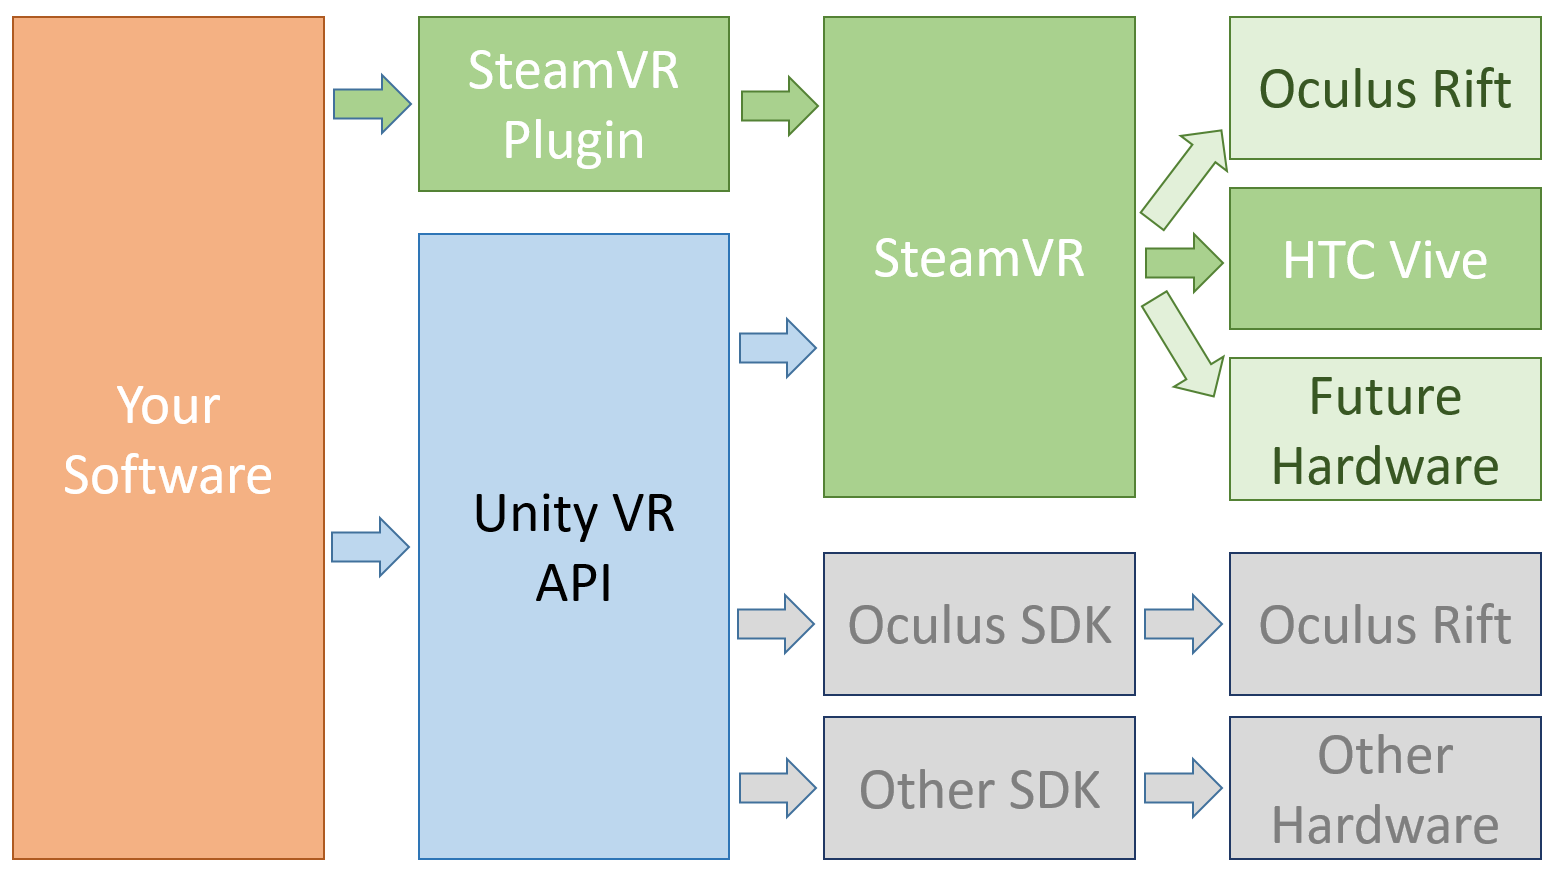
\includegraphics[width=14cm]{03_Figures/04_Valve/OpenVR_SteamVR_selected.png}
		\caption[Steam VR Unity Plugin]{Steam VR Unity Plugin (adopted from \cite{Valve2016})}
		\label{fig:steamvrselected}
	\end{center}
\end{figure}



%-----------------------------------
%	SUBSECTION 2
%-----------------------------------

\subsection{Data Model}

One of the main challenges is to get reasonable performance while working with a not so small data set (600+ entries as shown in Appendix \ref{AppendixA}) that can be filtered not only by year/month/day but also by several different categories atop of that. In order to not always filter through the whole data set, it will be split up in smaller parts that contain only data for a specific month in a specific year. While reading in the CSV file, multiple instances of the \textit{[System.Data.DataTable]} class are created and stored with the unique key \textit{[$<$year$>$-$<$month$>$]} in a \textit{[System.Collections.Generic.Dictionary]} which is the C\# equivalent of a HashMap in Java. For the filtering of the DataTable, the \textit{[System.Data.DataView]} class is used which itself does not store data but represents a connected view of a DataTable. While this already helps with the performance, as soon as the category filtering comes in place it still is relatively slow as all twelve months need to be updated. \newline
To at least partially address this problem, a caching of the filtered data for the bar charts and table has been considered. For this, another unique key had to be defined in the form of \textit{[$<$year$>$-$<$month$>$-$<$day$>$-$<$binaryCategory$>$]}. The "binaryCategory" is a binary state representation of all \textbf{eleven} categories where each one of them is either represented as a '0' (inactive) or a '1' (active). Following are some example to indicate how certain situations can be represented:
\begin{itemize}[noitemsep,nolistsep]
	\item 2016-0-0-00000000000 \textit{(only year selected and all categories inactive)}
	\item 2016-3-0-11111111111 \textit{(single month selected and all categories active)}
	\item 2016-8-27-11100010101 \textit{(selection of a specific day with different category states)}
\end{itemize}
With eleven categories, over 2'048 different combinations can be made across them. If this is considered for a whole year (365 days) there are a staggering amount of 747'520 different key-combinations, which makes it impractical to try to pre-cache every single combination. Due to this an on-demand cache is implemented to at least massively reduce the loading times of previously selected combinations. Listing \ref{lst:csharpdictionarydefinition} shows all definitions for the different containers that hold the information during runtime. \textit{dataTableDict} stores the different \textit{DataTable}s per month, \textit{chartValuesDict} and \textit{chartLabelsDict} contain the labels and values for all bar charts with their long unique key, and finally \textit{tableRowsDict} which helds the information for the table again with the long unique key. All these attributes are defined in the \textit{DataViewManager.cs} class that is referenced in the \textit{SceneManager.cs} class which is a Singleton instance and thus is guaranteed to only exist once in runtime and is also always accessible from any other script.
\begin{lstlisting}[caption={Dictionary definitions for data storage during runtime}, label={lst:csharpdictionarydefinition}]
public Dictionary<string, DataTable> dataTableDict;
private Dictionary<string, float[]> chartValuesDict;
private Dictionary<string, string[]> chartLabelsDict;
private Dictionary<string, List<string[]>> tableRowsDict;
\end{lstlisting}


%-----------------------------------
%	SUBSECTION 3
%-----------------------------------

\subsection{Code Structure}

It is important to have an effective and clean code structure that reflects the different layers which all together become the software itself. The following Figure \ref{fig:unitycodestructure} shows the project structure in Unity 3D while Table \ref{tbl:codestructuredesc} explains this in more detail. The structure follows some best practices that are also applied in SteamVR and \gls{vrtk}.
\begin{figure}[h]
	\begin{center}
		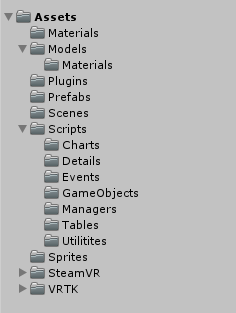
\includegraphics[width=7cm]{03_Figures/08_Development/CodeStructure.png}
		\caption{Prototype project structure in Unity 3D}
		\label{fig:unitycodestructure}
	\end{center}
\end{figure}


\begin{longtable}{ | p{3cm} | p{11cm} |}
	\hline
	\textbf{Folder} & \textbf{Description} \\
	\hline
	\endfirsthead % Line(s) to appear as head of the table on the first page
	\multicolumn{2}{c}%
	{\tablename\ \thetable\ -- \textit{Continued from previous page}} \\
	\hline
	\textbf{Folder} & \textbf{Description} \\
	\hline
	\endhead % Line(s) to appear at top of every page (except first)
	\hline
	\multicolumn{2}{r}{\textit{Continued on next page}} \\
	\endfoot % Last line(s) to appear at the bottom of every page (except last)
	\endlastfoot % Last line(s) to appear at the end of the table
	\hline
		\textbf{Assets} &
		This is the base-folder which is given by Unity 3D itself. It contains all files that are either required or created by the developer. \\
	\hline
		Materials &
		The Materials folder contains material (*.mat) files that can be applied to 2D/3D objects. \\
	\hline
		Models &
		In this folder, all models created in Blender (*.blend) are stored which can be dragged into the 3D scene. \\
	\hline
		\textrightarrow{} Materials &
		Contains all model-specific material (*.mat) files that are created in Blender. \\
	\hline
		Plugins &
		Additional C\# plugins (*.dll) are put here such as System.Data.dll which allows the processing and manipulation of data files. \\
	\hline
		Prefabs &
		In this folder, fully configured GameObjects can be stored (*.prefab) and instantiated multiple times. All instances inherit the base configuration and changes can be applied to all of them very easily. The individual bars of the bar chart are an example of such a prefab. \\
	\hline
		Resources &
		The base folder for where all additional resources are located. \\
	\hline
		\textrightarrow{} CSV &
		In this sub-folder, the data file (*.csv) which contains the categorized financial expenses is located. \\
	\hline
		Scenes &
		Within one Unity project, there can be multiple scenes (*.unity), which can be seen some kind of broken down parts of bigger applications where multiple different locations are available. In this prototype there is only a single scene used. \\
	\hline
		Scripts &
		The base folder for all C\# scripts (*.cs) that are used. \\
	\hline
		\textrightarrow{} Charts &
		Contains all scripts that are related to the functionality of the bar charts. \\
	\hline
		\textrightarrow{} Details &
		All scripts related to the detail view where all information about a financial transaction are shown. \\
	\hline
		\textrightarrow{} Events &
		Custom events that can be triggered from the gesture controllers are located here. \\
	\hline
		\textrightarrow{} GameObjects &
		Scripts related to specific game objects (e.g. the category icons) are stored in this folder. \\
	\hline
		\textrightarrow{} Managers &
		Contains two manager classes that hold together the whole information of the running scene and the stored/cached data. \\
	\hline
		\textrightarrow{} Tables &
		All scripts that are related to the table which shows a list of financial transactions \\
	\hline
		\textrightarrow{} Utilities &
		All other utility classes such as a unified Debugging/Logging. \\
	\hline
		Sprites &
		In this folder any kind of images (e.g. *.png) are stored that are used within the application, such as the threshold line for the bar charts. \\
	\hline
		SteamVR &
		Here all folders and files from the SteamVR plugin are copied to. It also contains certain prefabs that control the \gls{hmd} and geture controllers. \\
	\hline
		\gls{vrtk} &
		Similar to the SteamVR folder, all scripts and prefabs from \gls{vrtk} are located under this folder. \\
	\hline
	\caption{Explanation of prototype project structure in Unity 3D}
	\label{tbl:codestructuredesc}
\end{longtable}


%----------------------------------------------------------------------------------------
%	SECTION 4
%----------------------------------------------------------------------------------------

\section{Implementation of Views and Interaction}

In this chapter, an overview of all the views and their usage is provided, as well the interaction between them is discussed.

%-----------------------------------
%	SUBSECTION 1
%-----------------------------------
\subsection{Views / UI}

The following list of views refers back to the Suggestion chapter where the Navigation Map (Figure \ref{fig:navigationmap}) and Interaction Map (Figure \ref{fig:interactionmap}) are described. For each view a short explanation about its purpose is provided, alongside some design aspects from the development, and a screenshot that shows the view of final prototype application.

%-----------------------------------
%	SUBSUBSECTION 1
%-----------------------------------
\subsubsection{View 1: Year Overview}

\textbf{Purpose of view:}


\textbf{Possible Navigation:}


%-----------------------------------
%	SUBSUBSECTION 2
%-----------------------------------
\subsubsection{View 2: Month Overview}

\textbf{Purpose of view:}


\textbf{Possible Navigation:}


%-----------------------------------
%	SUBSUBSECTION 3
%-----------------------------------
\subsubsection{View 3: Year Selection}

\textbf{Purpose of view:}


\textbf{Possible Navigation:}


%-----------------------------------
%	SUBSUBSECTION 4
%-----------------------------------
\subsubsection{View 4: Categories Filtering}

\textbf{Purpose of view:}


\textbf{Possible Navigation:}


%-----------------------------------
%	SUBSUBSECTION 5
%-----------------------------------
\subsubsection{View 5: Fin. Transactions Overview}

\textbf{Purpose of view:}


\textbf{Possible Navigation:}


%-----------------------------------
%	SUBSUBSECTION 6
%-----------------------------------
\subsubsection{View 6: Fin. Transaction Details}

\textbf{Purpose of view:}


\textbf{Possible Navigation:}


%-----------------------------------
%	SUBSECTION 2
%-----------------------------------
\subsection{Interactions}

tbd


TODO:
5. implementation of views and navigation
- Code Structure?
- (Unity) Object Design
- (Unity) Script Design
- Important Code Snippets?
- Screenshots



Category Selection - waiting for data load --> coloring!
\gls{mdg} 1 that requires a high interactivity with tightly coupled actions/reactions.


%----------------------------------------------------------------------------------------
%	SECTION 5
%----------------------------------------------------------------------------------------

\section{Conclusion}


TODO:
6. Conclusion


%-----------------------------------
%	SUBSECTION 1
%-----------------------------------
\subsection{Unity 3D}


%-----------------------------------
%	SUBSECTION 2
%-----------------------------------
\subsection{\gls{vrtk}}


%% IDEA FOR PROTOTYPE

% - Start with a small table on which a house etc is visualized. floating above is year (+month)
% + Each object represents one category from the financial expenses.
% - maybe size indicates the overall amount?
% - The colours depends on the difference between my planned expenses (or average expenses) and the actual expenses. less = green, about the same = yellow-(green-)ish, slightly above = orange, above = red.
% - By clicking on one of the objects, it gets highlighted and a line-chart appears showing the expenses
% A) show individual transactions for the given month up until the threshold
% B) show individual months until the threshold (+forecast?)
% - show multiple lines for the different sub-categories (enable/disable) plus the total
% - clicking on an entry of the line chart displays details about transaction (amount, location), or the month (amount) in an overlay
% - switching between single-month and year view by... using the touchpad (up/down clicks)
% - navigating through months/years by... a using the touchpad! (left/right clicks)
% - resetting the view to start by... clicking on the select button

% - maybe outside as rotating rings: the individual bank accounts?
